\section{Overview}
The architecture of uniRDMA is shown in Figure~\ref{fig:framework-overview}. uniRDMA mainly consists of vRNIC, which is a para-virtualization device for guest, and the management layer(虚拟层暂定为管理层). Besides, some modifications are made to RDMA user library and device specific drivers for cooperating with uniRDMA.

(1) vRNIC frontend and backend: vRNIC frontend is as the device driver of hosts' backend. It cooperates with modified verbs and device-specific libraries and forwards serial commands to backend. In specific, the frontend is in kernel for VMs. vRNIC backend is as virtual device in host user space. It execute received commands. To achieve high performance, the control path and data path are separate in vRNICs. For data path, vRNIC frontend does not forwards RDMA commands, and directly use the mapped RDMA resources (e.g. QPs or MRs). The resources are mapped to backend by shared memory.

(2) Management Layer: To make a centralized management, a management center connect with each host's uniRDMA backend. The management mainly includes vRNIC device management and network management. For device management, the layer coordinates the hardware resources (e.g. VFs in SR-IOV) to achieve the hardware-support functions effectively, e.g. performance isolation. For network management, the layer can construct a virtual RDMA network by software methods, including configuring each vRNIC address, defining routing rules and maintaining the mapping for vRNIC connections. (包含设备管理和网络管理两个部分,设备管理主要是协调硬件虚拟化VF资源,网络管理是纯软件实现,包括配置vRNIC地址和路由规则等)

Besides, to support transparency for applications in guest, we modified the verbs library and hardware-specific libraries in guest. After modification, the RDMA commands can be forwarded to vRNIC frontends. Also, the memory of RDMA resources (e.g. QPs) can be backend with our shared memory. (必须修改设备相关库,RDMA QP资源的内存才能够用我们的共享内存去支持)

\begin{figure}[!ht]
	\centering
	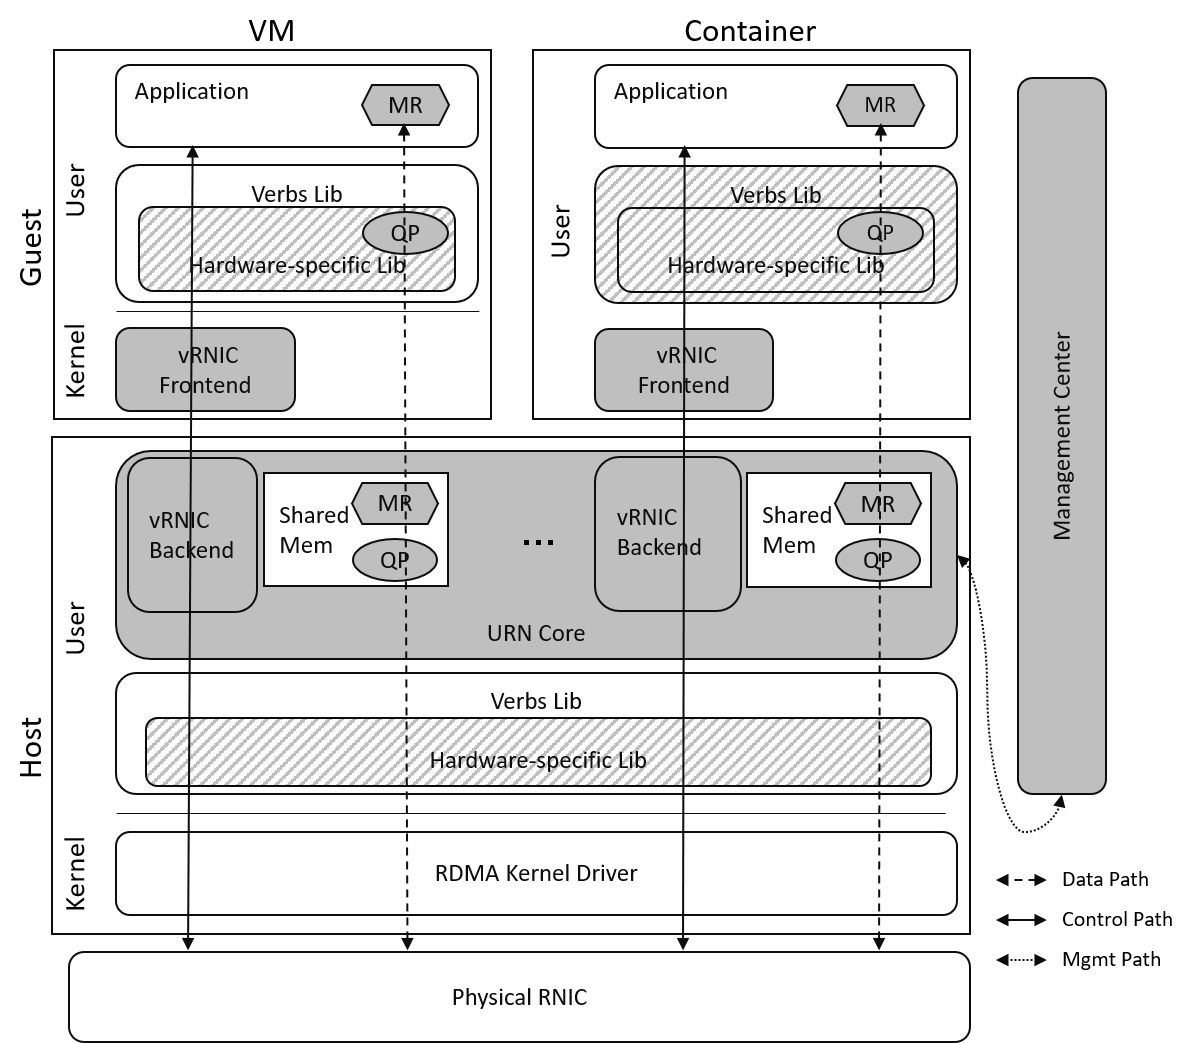
\includegraphics[width=1\linewidth]{images/framework-overview.png}
	\caption{uniRDMA Framework Overview}
	\label{fig:framework-overview}
\end{figure}